\documentclass[12pt]{article}

\usepackage{times, graphicx}
\usepackage{natbib}
\bibpunct{(}{)}{;}{a}{}{,}

\usepackage{geometry}
\geometry{verbose,tmargin=1in,bmargin=1in,lmargin=1in,rmargin=1in}


\usepackage{algpseudocode}
\algblock{ParFor}{EndParFor}
\algnewcommand\algorithmicparfor{\textbf{parallel for}}
\algnewcommand\algorithmicpardo{\textbf{do}}
\algnewcommand\algorithmicendparfor{\textbf{end\ parallel for}}
\algrenewtext{ParFor}[1]{\algorithmicparfor\ #1\ \algorithmicpardo}
\algrenewtext{EndParFor}{\algorithmicendparfor}

\usepackage{xcolor}

\newcommand{\matern}{Mat\'{e}rn}
\newcommand{\proglang}[1]{\textbf{\texttt{#1}}}
\newcommand{\pkg}[1]{\textbf{#1}}
\newcommand{\code}[1]{\texttt{#1}}
\newcommand{\bm}[1]{\mbox{\boldmath $#1$}}
\newcommand\T{\rule{0pt}{3.5ex}}

\begin{document}

\author{Christopher J. Paciorek, University of California, Berkeley\\
  Benjamin Lipshitz, University of California, Berkeley\\
Wei Zhuo, Georgia Institute of Technology\\
 Prabhat, Lawrence Berkeley National Laboratory\\
 Cari G. Kaufman, University of California, Berkeley\\
Rollin C. Thomas, Lawrence Berkeley National Laboratory}

\title{Parallelizing Gaussian Process Calculations in \proglang{R}}

\maketitle

\begin{abstract}
  We consider parallel computation for Gaussian process calculations
  to overcome computational and memory constraints 
  on the size of datasets that can be analyzed.  Using a hybrid parallelization approach that uses both
  threading (shared memory) and message-passing (distributed memory), we
  implement the core linear algebra operations used in spatial
  statistics and Gaussian process regression in an \proglang{R} package called \pkg{bigGP} that relies on \proglang{C} and \pkg{MPI}. The approach divides the covariance matrix into blocks such that the computational
load is balanced across processes while communication between processes is limited. The package
  provides an API enabling \proglang{R} programmers to implement Gaussian process-based
  methods by using the distributed linear algebra operations without any \proglang{C} or \pkg{MPI} coding.
  We illustrate the approach and software by analyzing an astrophysics
  dataset with $n=67,275$ observations.
\end{abstract}


\section{Introduction}
Gaussian processes are widely used in statistics and machine learning
 for spatial and spatio-temporal modeling \citep{Bane:etal:2003}, design and analysis of computer experiments \citep{Kenn:OHag:2001}. \cite{Rasm:Will:2006} illustrate the use of these processes in nonparametric regression. 
One popular example is the spatial statistics method of kriging, which is equivalent to conditional expectation under a Gaussian process model for the  unknown spatial field.
However standard implementations of Gaussian process-based methods 
are computationally intensive because they involve calculations with
covariance matrices of size $n$ by $n$ where $n$ is the number of
locations with observations. In particular the computational
bottleneck is generally the Cholesky decomposition of the covariance
matrix, whose computational cost is of order $n^3$. 

For example, a
basic spatial statistics model (in particular a geostatistical model) can be specified in a hierarchical fashion as
\begin{eqnarray}
\bm{Y}|\bm{g},\bm{\theta} & \sim & \mathcal{N}(\bm{g},\bm{C}_y(\bm{\theta})) \nonumber\\
\bm{g}|\bm{\theta} & \sim & \mathcal{N}(\bm{\mu}(\bm{\theta}),\bm{C}_g(\bm{\theta})),\label{eq:main}
\end{eqnarray}
 where $\bm{g}$ is a vector of latent spatial process values at the $n$ locations, $\bm{C}_y(\bm{\theta})$ is an error covariance matrix (often diagonal), $\mu(\bm{\theta})$ is the mean vector of the latent process, $\bm{C}_g(\bm{\theta})$ is the spatial covariance matrix of the latent process, and $\bm{\theta}$ is a vector of unknown parameters.
We can marginalize over $\bm{g}$ in (\ref{eq:main}) to obtain the marginal likelihood,
\[
\bm{Y}|\bm{\theta} \sim\mathcal{N}(\bm{\mu}(\bm{\theta}), \bm{C}(\bm{\theta})),\]
where $\bm{C}(\bm{\theta}) = \bm{C}_y(\bm{\theta}) + \bm{C}_g(\bm{\theta})$. 
This gives us the marginal density,
\[f(\bm{y})\propto|\bm{C}(\bm{\theta})|^{-1/2}\exp\left\{
  -\frac{1}{2}(\bm{y}-\bm{\mu}(\bm{\theta}))^{\top}(\bm{C}(\bm{\theta}))^{-1}(\bm{y}-\bm{\mu}(\bm{\theta}))\right\}, \]
which is maximized over $\bm{\theta}$ to find the maximum
likelihood estimator. At each iteration 
in the maximization, the expensive computations are to compute the entries of the matrix $\bm{C}(\bm{\theta})$ as a function of $\bm{\theta}$, calculate the Cholesky decomposition,
$\bm{LL}^{\top}=\bm{C}(\bm{\theta})$, and solve a system of
equations $\bm{L}^{-1}(\bm{y}-\bm{\mu}(\bm{\theta}))$ via a forwardsolve operation. Given the MLE, $\hat{\bm{\theta}}$,
one might then do spatial prediction, calculate the variance of the prediction, and simulate
realizations conditional on the data. These additional tasks involve the same expensive computations plus
a few additional closely-related computations.  

  This set of core
functions includes Cholesky decomposition, forwardsolve and backsolve, and crossproduct calculations. These functions, plus some auxiliary functions for communication of inputs
and outputs to the processes, provide an API through which an \proglang{R}
programmer can implement methods for Gaussian-process-based
computations. Using the API, we provide a set of methods for the
standard operations involved in kriging and Gaussian process
regression, namely 
\begin{itemize}
\item likelihood optimization, 
\item prediction,
\item calculation of prediction uncertainty, 
\item unconditional simulation of
Gaussian processes, and 
\item conditional simulation given data.
\end{itemize}
These
methods are provided as \proglang{R} functions in the package. We
illustrate the use of the software for Gaussian process regression in
an astrophysics application.

We close this introduction by situating our software within the context of other software for Gaussian process modeling. A broad variety of software, both within and outside of \proglang{R}, is available for working with Gaussian processes, much of it implementing various approximate methods. However, there is little parallelized software for working with Gaussian processes without approximations. \proglang{R} provides a wide variety of tools for parallelization, best summarized in the High Performance Computing task view on CRAN, as well as a variety of tools for Gaussian process models. The Gaussian process-related packages available on CRAN do not provide parallelized software for exact calculations, with packages such as \pkg{mlegp} \citep{Danc:etal:2008}. Note that while our software is based upon the blocked approach of \pkg{ScaLAPACK} (Section~\ref{sec:block-chol}), we tailor the algorithm to achieve better load-balancing and limit communication for Cholesky factorization (Section~\ref{sec:our-alg}).
Looking outside of \proglang{R}, the \pkg{ScalaGAUSS} package \citep{scalaGauss} implements (in \proglang{C++} and \proglang{MATLAB}) likelihood maximization for Gaussian processes using a stochastic approximation to the likelihood that allows for optimization using matrix-vector calculations that are of order $n\log n$ \citep{Anit:etal:2012}.  Recent advances in communication-avoiding linear algebra \citep{BDHS11} in general, and especially for Cholesky decomposition \citep{GGSYTY12} may prove useful in speeding up parallel Gaussian process computation, but have not yet been incorporated into standard libraries like \pkg{ScaLAPACK}.




\section{Parallel algorithm and software implementation}

\subsection{Distributed linear algebra calculations}
\label{sec:block-chol}
Parallel computation can be done in both shared memory and distributed memory contexts. Each uses multiple CPUs. In a shared memory context (such as computers with one or more chips with multiple cores), multiple CPUs have access to the same memory and so-called `threaded' calculations can be done, in which code is written (e.g., using the \pkg{openMP} protocol \citep{openMP}) to use more than one CPU at once to carry out a task, with each CPU having access to the objects in memory. In a distributed memory context, one has a collection of nodes, each with their own memory. Any information that must be shared with other nodes must be communicated via message-passing, such as using the \pkg{MPI} standard. Our distributed calculations use both threading and message-passing to exploit the capabilities of modern computing clusters with multiple-core nodes.

We begin by describing a basic parallel Cholesky decomposition, sometimes known as Crout's algorithm, which is done on blocks of the matrix and is implemented in \pkg{ScaLAPACK}. Figure~\ref{fig:dependency-graph} shows a schematic of the block-wise Cholesky factorization, where the covariance matrix is divided into 6 blocks, a $B=3$ by $B=3$ array of blocks (storing only the lower blocks of the symmetric matrix). 

\begin{figure}
 \centering
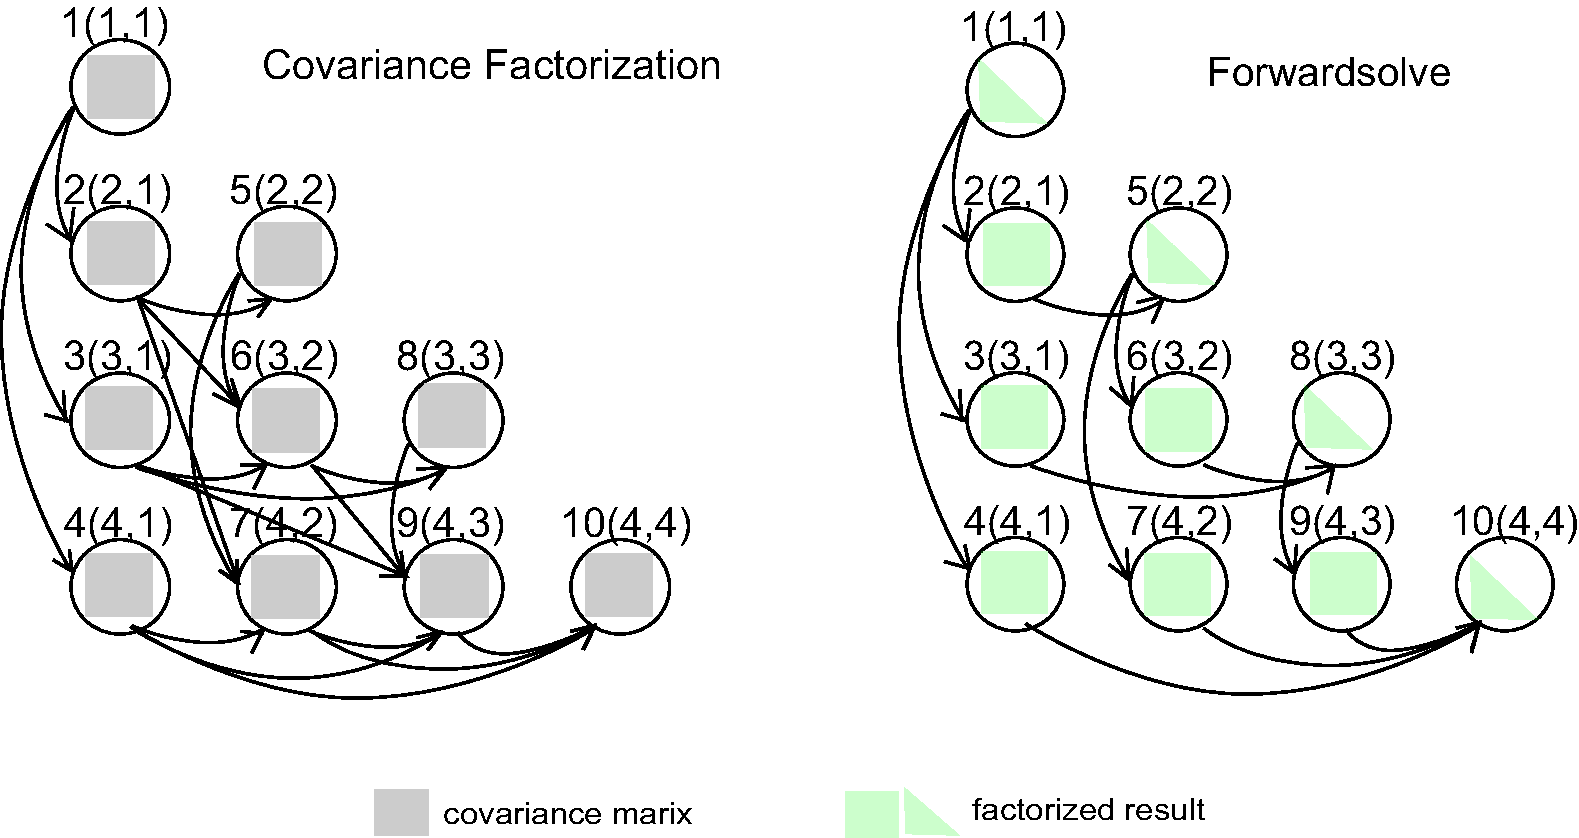
\includegraphics[scale=.5]{figs/dependency_h}
 \caption{
Diagram of the first steps in the distributed Cholesky factorization.  Arrows indicate dependencies between processes. Orange coloring indicates computations carried out in each step, and green indicates parts of the matrix that are completely factored as of the previous step. The labels of the form ``id(x,y)'' indicate the process ID and Cartesian coordinates of the process.\label{fig:dependency-graph}}
\end{figure}

% [insert refs 5,6,8,13 from ICDM paper as needed]

To specify the distributed algorithm, there are several choices to be made: the number of blocks, \(B\), how to distribute these blocks amongst computational processes, how to distribute these processes amongst the nodes, and how many nodes to use.  We discuss the tradeoffs involved in these choices next and the choices that our algorithm makes in Section~\ref{sec:our-alg}.


\subsection{Our algorithm}
\label{sec:our-alg}


We require that the number of processes is \(P=D(D+1)/2 \in \{1,3,6,10,15,\ldots\}\) for some integer value of \(D\).  We introduce another quantity \(h\) that determines how many blocks each process owns.  The number of blocks is given by \(B=hD\), and so the block size is
$\left\lceil\frac{n}{hD}\right\rceil,$
where \(n\) is the order of the matrix.  See Figure~\ref{fig:matrix-vary-h} for an example of the layout with \(D=4\) and either \(h=1\) or \(h=3\).  Each ``diagonal process'' has \(h(h+1)/2\) blocks, and each ``off-diagonal process'' has \(h^2\) blocks of the triangular matrix.

\begin{figure}
  \centering
  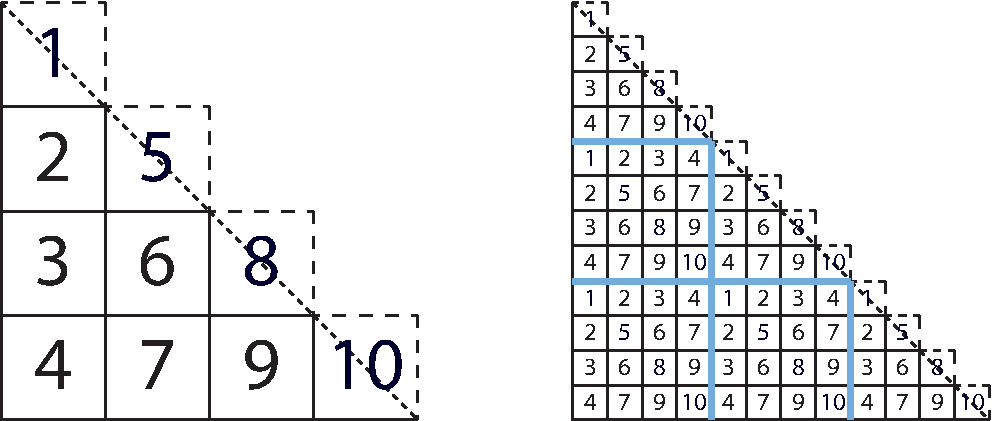
\includegraphics[scale=.75]{figs/vary-h}
  \caption{The matrix layout used by our algorithm with \(D=4\) and \(h=1\) (left) or \(h=3\) (right).  The numbers indicate which process owns a given block.  When \(h=1\), each of the 10 processes owns one block of the matrix.  When \(h=3\), the blocks are a third the size in each dimension.  The diagonal processes (1, 5, 8, 10) each own \(h(h+1)/2=6\) blocks, and the off-diagonal processes (2, 3, 4, 6, 7, 9) each own \(h^2=9\) blocks.}
  \label{fig:matrix-vary-h}
\end{figure}


Note that when \(h>1\), there are essentially two levels of blocking, indicated by the thin black lines and the thick blue lines in Figure~\ref{fig:matrix-vary-h}.  Our algorithm is guided by these blocks.  At a high level, the algorithm sequentially follows the Cholesky decomposition of the large (blue) blocks as described in the previous section.  Each large block is divided among all the processors, and all the processors participate in each step.  For example, the first step is to perform Cholesky decomposition on the first large block.  To do so, we follow exactly the \(h=1\) algorithm (making use of the Cartesian coordinate identification system indicated in Figure~\ref{fig:dependency-graph}):
\begin{algorithmic}[1]
\For{$i=1$ to $D$}
\State Processor $(i,i)$ computes the Cholesky decomposition of its block
\ParFor{$j=i+1$ to $D$}
\State Processor $(i,i)$ sends its block to processor $(j,i)$
\State Processor $(j,i)$ updates its block with a triangular solve
 \ParFor{$k=i+1$ to $D$}
 \If{$k\leq j$}
   \State Processor $(j,i)$ sends its block to processor $(j,k)$
 \Else
   \State Processor $(j,i)$ sends its block to processor $(k,j)$
 \EndIf
 \EndParFor
\EndParFor
\ParFor{$j=i+1$ to $D$}
 \ParFor{$k=j+1$ to $D$}
  \State Processor $(k,j)$ updates its block with a matrix multiplication
 \EndParFor
\EndParFor
\EndFor
\end{algorithmic}
The \(h=1\) algorithm is poorly load-balanced; for example going from $D=1$ to $D=2$ (one process to three processes), one would not expect any speedup because every operation is along the critical path.  However, because it is a small portion of the entire calculation for $h>1$, the effect on the total runtime is small.  Instead, most of the time is spent in matrix multiplications of the large blue blocks, which are well load-balanced.



\subsubsection{Memory use}
The number of informative entries in a triangular or symmetric \(n\times n\) matrix is \(n(n+1)/2\).  Ideally, it would be possible to perform computations even if there is only barely this much memory available across all the nodes, that is if there were enough memory for \(n(n+1)/(D(D+1))\) entries per node.  Our algorithm does not reach this ideal, but it has a small memory overhead that decreases as \(D\) or \(h\) increase. The maximum memory use is by the off-diagonal nodes that own \(h^2\) blocks.  Additionally, during the course of the algorithm they must temporarily store up to 4 more blocks.  Assuming for simplicity that $hD$ evenly divides $n$, the maximum memory use on a node is then
\begin{eqnarray}
M&\leq \left(\frac{n}{hD}\right)^2(h^2+4)=\frac{n(n+1)}{D(D+1)}\left(1+\frac{4nD+n^2h^2+4n-Dh^2}{Dh^2n+Dh^2}\right) \\&< \frac{n(n+1)}{D(D+1)}\left(1+\frac{4}{h^2}+\frac{1}{D}+\frac{4}{Dh^2}\right).
\end{eqnarray}
For example when \(h=3\) and \(D=4\), the memory required is about 1.8 times the memory needed to hold a triangular matrix.  Increasing \(h\) and \(D\) decreases this overhead factor toward 1.

\textcolor{red}{would we like two more brief sections that work out the math for load balance and for communication cost? Also do we prefer precise calculations, as above, or asymptotic ones}


\subsection[The bigGP R package]{The \pkg{bigGP} \proglang{R} package}

\subsubsection{Overview}


The \proglang{R} package \pkg{bigGP} implements a set of core functions, all in a distributed fashion, that are useful for a variety of Gaussian process-based computational tasks. In particular we provide Cholesky factorization, forwardsolve, backsolve and multiplication operations, as well as a variety of auxiliary functions that are used with the core functions to implement high-level statistical tasks.  We also provide additional \proglang{R} functions for distributing objects to the processes, managing the objects, and collecting results at the master process.

This set of \proglang{R} functions provides an API for \proglang{R} developers. A developer can implement new tasks entirely in \proglang{R} without needing to know or use \proglang{C} or \pkg{MPI}. Indeed, using the API, we implement standard Gaussian process tasks: log-likelihood calculation, likelihood optimization, prediction, calculation of prediction uncertainty, unconditional simulation of Gaussian processes, and simulation of Gaussian process realizations conditional on data. Distributed construction of mean vectors and covariance matrices is done using user-provided \proglang{R} functions that calculate the mean and covariance functions given a vector of parameters and arbitrary inputs. 

\subsubsection{API}

The API consists of 
\begin{itemize}
\item basic functions for listing and removing objects on the slave processes and copying objects to and from the slave processes: \code{remoteLs}, \code{remoteRm}, \code{push}, \code{pull};
\item functions for determining the lengths and indices of vectors and matrices assigned to a given slave process: \code{getDistributedVectorLength},\\\code{getDistributedTriangularMatrixLength},\\\code{getDistributedRectangularMatrixLength}, \code{remoteGetIndices};
\item functions that distribute and collect objects to and from the slave processes, masking the details of how the objects are divided amongst the processes: \code{distributeVector}, \\\code{collectVector}, \code{collectDiagonal}, \code{collectTriangularMatrix},\\\code{collectRectangularMatrix}; and
\item functions that carry out linear algebra calculations on distributed vectors and matrices: \\\code{remoteCalcChol}, \code{remoteForwardsolve}, \code{remoteBacksolve}, \\\code{remoteMultChol}, \code{remoteCrossProdMatVec}, \code{remoteCrossProdMatSelf}, \\\code{remoteCrossProdMatSelfDiag}, \code{remoteConstructRnormVector}, and \code{remoteConstructRnormMatrix}. In addition there is a generic \code{remoteCalc} function that can carry out an arbitrary function call with either one or two inputs. 
\end{itemize}

The package must be initialized after loading, which is done with the
\code{bigGP.init} function. During initialization, slave processes are
spawned and \proglang{R} packages loaded on the slaves, parallel
random number generation is set up, and blocks are assigned to slaves,
with this information stored on each slave process in the
\code{.bigGP} object. Users need to start \proglang{R} in such a way
(e.g., through a queueing system or via \code{mpirun}) that $P$ slave
processes can be initialized, plus one for the master process, for a
total of $P+1$. $P$ should be such that $P = D(D+1)/2$ for integer
$D$, i.e., $P \in {3,6,10,15,\ldots}$. One may wish to have one
process per node, with threaded calculations on each node via a
threaded \pkg{BLAS}, or one process per core (in particular when a
threaded \pkg{BLAS} is not available). The determination of the number
of cores per process is system-specific and not set at the level of \proglang{R}
or by \pkg{bigGP}. Rather, the user must request a total number of
processes and cores per process via whatever queueing system is in
place (if any) on the system they are using or by specifying the hosts
if simply using \code{mpirun}.  We note that apart from requesting
resources from the system, the user must specify only a single number,
$P$, in \proglang{R}.


\subsubsection{Kriging implementation}

The kriging implementation is built around two reference classes. 

The first is a \code{krigeProblem} class that contains metadata about the problem and manages the analysis steps. To set up the problem and distribute inputs to the processes, one instantiates an object in the class. The metadata includes the block replication factors and information about which calculations have been performed and which objects are  up-to-date (i.e., are consistent with the current parameter values). This allows the package to avoid repeating calculations when parameter values have not changed. Objects in the class are stored on the master process. 


\subsubsection{Using the API}

To extend the package to implement other Gaussian process methodologies, the two key elements are construction of the distributed objects and use of the core distributed linear algebra functions. Construction of the distributed objects should mimic the\\\code{localKrigeProblemConstructMean} and \code{localKrigeProblemConstructCov} functions in the package. 
\section{Timing results}
\label{sec:results}

We focus on computational speed for the Cholesky factorization, as this generally dominates the computational time for Gaussian process computations. We run the code underlying the package as a distributed \proglang{C} program, as \proglang{R} serves only as a simple wrapper that calls the local Cholesky functions on the worker processes via the \code{mpi.remote.exec} function. We use Hopper, a Cray system hosted at the National Energy Research Scientific Computing center (NERSC). Each Hopper node consists of two 12-core AMD ``MagnyCours'' processors with 24 GB of memory.  Hopper jobs have access to a dedicated Cray Gemini interconnect to obtain low-latency and high bandwidth inter-process communication.  While Hopper has 24 cores per node, each node is divided into 4 NUMA regions each with 6 cores; in our experiments we try running one process per node, one process per NUMA region (4 per node), or one process per core (24 per node).

We start by considering timing as a function of the size of the problem, illustrating that our approach greatly reduces computational time and that it allows one to do computations for matrices too large to work with on an individual machine. We then consider the choice of $h$ and compare our implementation with \pkg{ScaLAPACK}, illustrating that our implementation is equivalent in terms of timing. Next we explore the question of how to assign one's available cores: fewer processes and more cores per process or the reverse. Finally, we consider the use of GPUs.

\subsection{Timing with increasing problem size and comparison with a naive implementation}
As the matrix size \(n\) increases, the arithmetic count of computations required for Cholesky decomposition increases as a function of \(n^3\).  For small problem sizes, this increase is mitigated by the greater efficiency in computing with larger matrices.  Figure~\ref{fig:vary-n} shows how runtime varies with \(n\).

As a practical illustration, if 100 Cholesky decompositions were required for likelihood optimization for a problem with $n=8192$, one could carry out the optimization using our implementation with six cores on Hopper in approximately 440 seconds. This is comparable to using a fast threaded \pkg{BLAS} to do a standard Cholesky on a desktop machine. In particular using \proglang{R} on a desktop Linux machine with 16 GB RAM and 8 cores linked to \pkg{openBLAS} or on a Mac Mini with 8 GB RAM and 4 cores linked to the \pkg{vecLib} \pkg{BLAS}, the 100 decompositions would take approximately 500 and 610 seconds respectively. In contrast, by using 816 cores on Hopper, computational time is reduced to 40 seconds for 100 decompositions. Furthermore, with 816 cores, such an optimization with $n=32768$ would take approximately 950 seconds with our implementation, but neither of the desktop machines could factorize the matrix because of memory constraints. 

\begin{figure}
  \centering
  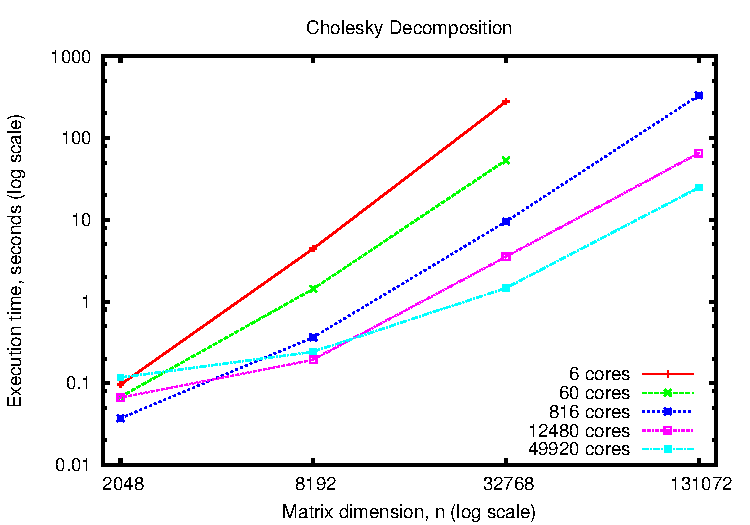
\includegraphics[scale=1]{figs/plotb}
  \caption{Runtimes as a function of \(n\) for Cholesky decomposition on Hopper, for a variety of numbers of cores.  For 49920 cores, we used 24 cores per process; in the other cases we used 6 cores per process. For each data point, we use the optimal value of \(h\), as determined in Section~\ref{sec:choiceH}. }
  \label{fig:vary-n}
\end{figure}

\subsection[Choice of h and comparison to ScaLAPACK]{Choice of $h$ and comparison to \pkg{ScaLAPACK}} \label{sec:choiceH}
In Figure~\ref{fig:vary-h} we compare the performance at different values of \(h\).  One notable feature is that for \(h=1\) there is no performance improvement in increasing from \(P=1\) to \(P=3\), because there is no parallelism.  Allowing larger values of \(h\) makes a speedup possible with \(P=3\).  Generally, larger values of \(h\) perform best when \(P\) is small, but as \(P\) grows the value of \(h\) should decrease to keep the block size from getting too small.

Figure~\ref{fig:vary-h} also compares our performance to \pkg{ScaLAPACK}, a standard distributed-memory linear algebra library.  Performance for \pkg{ScaLAPACK} (using the optimal block size) and our algorithm (using the optimal value of \(h\)) is similar.  We are thus able to get essentially the same performance on distributed linear algebra computations issued from \proglang{R} with our framework as if the programmer were working in \proglang{C} and calling \pkg{ScaLAPACK}.

\begin{figure}
  \centering
  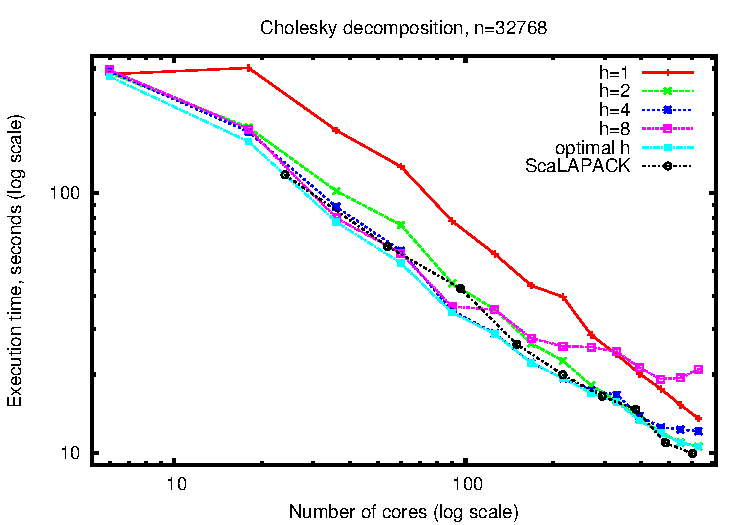
\includegraphics[scale=1]{figs/plota}
  \caption{Runtimes for \(32768\times32768\) Cholesky decomposition on Hopper with various values of $h$ using $6$ cores per process.  The last line shows \pkg{ScaLAPACK} as a benchmark.  The optimal value of $h$ was chosen by trying all values between 1 and 8.  The blocksize for \pkg{ScaLAPACK} corresponds to the best performance using a power of 2 blocks per process.}
  \label{fig:vary-h}
\end{figure}



\section{Astrophysics example}
\label{sec:example}


 
\subsection{Statistical model}

We model the flux measurements $Y_1, \ldots, Y_{67275}$ as being equal to a GP realization plus two error components: random effects for each phase (time point) and independent errors due to photon noise. We denote these three components by
$$Y_i = Z(t_i, w_i) + \alpha_{t_i} + \epsilon_{i},$$
where $t_i$ represents the time corresponding to $Y_i$ and $w_i$ the log wavelength, $\alpha_{t_i}$ is the random effect corresponding to time $t_i$, and $\epsilon_i$ is measurement error for the $i^{th}$ observation. The models for these components are
\begin{eqnarray*}
Z &\sim& GP(\mu(\cdot; \kappa, \lambda), \sigma^2 K(\cdot, \cdot; \rho_p, \rho_w))\\
\alpha_1, \ldots, \alpha_{25} &\stackrel{iid}{\sim}& N(0, \tau^2)\\
\epsilon_i &\sim& N(0, v_i), \quad \epsilon_1, \ldots, \epsilon_{67275} \mbox{ mutually independent.}
\end{eqnarray*}

$Z$ has mean function $\mu$, a function of time $t$ only, derived from a standard template Type Ia supernova spectral time series \citep{hsiao2007}, with $\kappa$ and $\lambda$ controlling scaling in magnitude and time. We take the correlation function, $K$, to be a product of two Mat\'ern correlation functions, one for both the phase and log wavelength dimensions, each with smoothness parameter $\nu=2$.  Note that the flux error variances $v_i$ are known, leaving us with six parameters to be estimated.

\subsection[R code]{\proglang{R} code}
For this problem we chose $P=465$, requesting $466$ processes (including one for the master) with $6$ cores per process on Hopper. In the \proglang{R} code, the first steps are to load the package, set up the inputs to the mean and covariance functions, and initialize the kriging problem object, called \code{prob}. Note that in this case the mean and covariance functions are provided by the package, but in general these would need to be provided by the user. 
\begin{verbatim}
R> library("bigGP")

R> nProc <- 465
R> n <- nrow(SN2011fe)
R> m <- nrow(SN2011fe_newdata)
R> nu <- 2
R> inputs <- c(as.list(SN2011fe), as.list(SN2011fe_newdata), nu = nu)

R> prob <- krigeProblem$new("prob", numProcesses = nProc, h_n = NULL, 
   h_m = NULL, n = n, m = m, meanFunction = SN2011fe_meanfunc, 
   predMeanFunction = SN2011fe_predmeanfunc, 
   covFunction = SN2011fe_covfunc, 
   crossCovFunction = SN2011fe_crosscovfunc, 
   predCovFunction = SN2011fe_predcovfunc, inputs = inputs, 
   params = SN2011fe_initialParams, data = SN2011fe$flux, 
   packages = 'fields', parallelRNGpkg = "rlecuyer")
\end{verbatim}
We then maximize the log likelihood, followed by making the kriging predictions and generating a set of 1000 realizations from the conditional distribution of $Z$ given the observations and fixing the parameters at the maximum likelihood estimates. The predictions and realizations are over a grid, with days ranging from -15 to 24 in increments of 0.5 and wavelengths ranging from 5950 to 6300 in increments of 0.5. The number of prediction points is therefore $79 \times 701 = 55379$.
\begin{verbatim}
R> prob$optimizeLogDens(method = "L-BFGS-B", verbose = TRUE, 
    lower = rep(.Machine$double.eps, length(SN2011fe_initialParams)), 
    control = list(parscale = SN2011fe_initialParams))

R> pred <- prob$predict(ret = TRUE, se.fit = TRUE, verbose = TRUE)
R> realiz <- prob$simulateRealizations(r = 1000, post = TRUE, 
      verbose = TRUE)

\end{verbatim}

\subsection{Results}

The MLEs are $\hat\sigma^2 = 0.0071$, $\hat\rho_p = 2.33$, $\hat\rho_w = 0.0089$, $\hat\tau^2 = 2.6\times 10^{-5}$, and $\hat\kappa = 0.33$. These are calculated from the 1000 sampled posterior realizations of $Z$. For each realization, we calculate the minimizing wavelength for each time point. 

Unrelated results are in Table \ref{tab:results}.
\begin{table}[!t]
\caption{Some results are here.}
%\vspace{.15in}
\begin{center}
\begin{tabular}{lc||c|cc|cc||c|cc|cc}
\hline
&& \multicolumn{5}{c||}{\textbf{Median absolute error}}& \multicolumn{5}{c}{\textbf{Median relative error}}\\
 & $n$ & M1 & M2 & (p) & M3 & (p) & M1 & M2 & (p) & M3 & (p) \\ 
  \hline
  \multicolumn{12}{l}{\textbf{\underline{Test 1: Holding out all studies from 10\% of countries}}} \T \\
mean \textsc{haz} & 181 & 0.21 & 0.20 & 0.16 & 0.28 & 0.00 & 0.15 & 0.14 & 0.56 & 0.19 & 0.00 \\ 
  \%\textsc{haz}$<$-2 & 292 & 6.02 & 5.94 & 0.36 & 8.05 & 0.00 & 0.17 & 0.17 & 0.19 & 0.25 & 0.00 \\ 
  \%\textsc{haz}$<$-3 & 202 & 3.62 & 3.40 & 0.57 & 4.12 & 0.00 & 0.27 & 0.26 & 0.26 & 0.30 & 0.00 \\ 
  \multicolumn{12}{l}{\textbf{\underline{Test 2: Holding out mean and \%$<$-3 when \%$<$-2 is known}}} \T \\
mean \textsc{haz} & 83 & 0.10 & 0.16 & 0.00 & 0.10 & 0.72 & 0.10 & 0.15 & 0.00 & 0.10 & 0.89 \\ 
 \%\textsc{haz}$<$-3 & 111 & 1.76 & 1.86 & 0.00 & 1.76 & 0.19 & 0.16 & 0.19 & 0.01 & 0.16 & 0.30 \\ 
   \hline
\label{tab:results}
\end{tabular}
\end{center}
\end{table}

\clearpage
\newpage
\begin{table}
\caption{Results for spatial simulation (1,000 Monte Carlo simulations for each scenario and 100 bootstrap samples).  
The average
out-of-sample $R^2$ is given in parentheses for each exposure model.  The first column is the relative bias in estimating $\beta=0.1$.  
This is the same for $\sigma^2=200$ and $\sigma^2=10$ and is estimated from 100,000 Monte Carlo
samples, resulting in negligible Monte Carlo error.
The final six columns show the standard deviation, average estimated standard error, and 95$\%$ confidence interval coverage, separately for 
$\sigma_\epsilon^2=200$ and $\sigma_\epsilon^2=10$.}
\small
\centering

\begin{tabular}{lrrrrrrr}
\noalign {\vspace{0.05cm}}
&&\multicolumn{3}{c}{$\sigma^2_\theta=200$}&\multicolumn{3}{c}{$\sigma^2_\theta=10$}\\
&\textrm{Rel Bias}&\textrm{SD}&\textrm{E(SE)}&\textrm{Cov}&\textrm{SD}&\textrm{E(SE)}&\textrm{Cov}\\
\hline
\noalign {\vspace{0.05cm}}
\textrm{Scenario }1\\
\hline
\noalign {\vspace{0.05cm}}
\textrm{5 degrees of freedom }(0.75)\\
\noalign {\vspace{0.05cm}}
\quad \textrm{no correction}&-0.027&0.084&0.083&94\%&0.02&0.019&93\%\\
\quad \textrm{bootstrap standard error only}&-0.027&0.084&0.084&95\%&0.02&0.021&95\%\\
\quad \textrm{bias correction only}&-0.009&0.086&0.083&94\%&0.021&0.019&93\%\\
\quad \textrm{bias correction + bootstrap}&-0.009&0.086&0.086&95\%&0.021&0.021&96\%\\
\noalign {\vspace{0.05cm}}
\textrm{10 degrees of freedom }(0.79)\\
\noalign {\vspace{0.05cm}}
\quad \textrm{no correction}&-0.039&0.08&0.08&95\%&0.019&0.018&93\%\\
\quad \textrm{bootstrap standard error only}&-0.039&0.08&0.082&96\%&0.019&0.027&98\%\\
\quad \textrm{bias correction only}&-0.025&0.081&0.08&94\%&0.019&0.018&93\%\\
\quad \textrm{bias correction + bootstrap}&-0.025&0.081&0.088&97\%&0.019&0.03&99\%\\
\hline
\noalign {\vspace{0.05cm}}
\textrm{Scenario }2\\
\hline
\noalign {\vspace{0.05cm}}
\textrm{5 degrees of freedom }(0.42)\\
\noalign {\vspace{0.05cm}}
\quad \textrm{no correction}&-0.125&0.099&0.096&94\%&0.025&0.022&87\%\\
\quad \textrm{bootstrap standard error only}&-0.125&0.099&0.097&95\%&0.025&0.026&90\%\\
\quad \textrm{bias correction only}&-0.049&0.108&0.096&93\%&0.028&0.022&86\%\\
\quad \textrm{bias correction + bootstrap}&-0.049&0.108&0.107&95\%&0.028&0.03&94\%\\
\noalign {\vspace{0.05cm}}
\textrm{10 degrees of freedom }(0.59)\\
\noalign {\vspace{0.05cm}}
\quad \textrm{no correction}&-0.102&0.087&0.085&93\%&0.021&0.019&88\%\\
\quad \textrm{bootstrap standard error only}&-0.102&0.087&0.085&94\%&0.021&0.03&94\%\\
\quad \textrm{bias correction only}&-0.061&0.091&0.085&92\%&0.023&0.019&88\%\\
\quad \textrm{bias correction + bootstrap}&-0.061&0.091&0.094&95\%&0.023&0.036&97\%\\
\end{tabular}

\label{tab:linear.sim}
\end{table}

\section{Discussion}

Our software allows one to carry out standard Gaussian process calculations, such as likelihood maximization, prediction, and simulation of realizations, off the shelf, as illustrated in the astrophysics example, in situations in which calculations using threaded linear algebra on a single computer are not feasible because the calculations take too long or use too much memory.  The software enables a user to implement standard models and related models without approximations. One limitation of our implementation is that we do not do any pivoting, so Cholesky factorization of matrices that are not numerically positive definite fails. This occurred in the example when simulating realizations on fine grids of wavelength and phase. 


\section*{Acknowledgments}

This work is supported by the Director, Office of Science, Office of Advanced Scientific Computing Research, of the U.S. Department of Energy under Contract No. AC02-05CH11231. This research used resources of the National Energy Research Scientific Computing Center.

\newpage

\bibliographystyle{plainnat}
\bibliography{refs}




\end{document}
